\documentclass[11pt]{article}
\usepackage[utf8]{inputenc}
\usepackage[noadjust]{cite}
\usepackage[english,greek]{babel}
\usepackage{csquotes}
\usepackage{etoolbox}
\usepackage{graphicx}
\usepackage{wrapfig}

\patchcmd{\thebibliography}{\section*{\refname}}{}{}{}

\usepackage{float}


\begin{document}
	
	
	\begin{titlepage}
		\begin{center}
			
\includegraphics[width=0.4\textwidth]{university}
			
			\vspace{0.1cm}
			
			\Large
			Τμήμα Μηχανικών Η/Υ και Πληροφορικής\\
			Πολυτεχνική Σχολή	
			
			\vspace{2.5cm}
			
			\huge
			\textbf{Το λογισμικό: μια πορεία 50 ετών και το μέλλον του}
			
			
			\vspace{4.0cm}
			\Large
			\textbf{ΝΙΚΟΛΑΟΣ ΓΕΩΡΓΟΠΟΥΛΟΣ-ΝΙΝΟΣ }
			\normalsize
			\underline{AM:1054385}
			
			\vfill
			Εργασία για το μάθημα Συγγραφή 
			και Παρουσίαση Τεχνικών Κειμένων
			
			\vspace{0.8cm}
			
			\Large
			19 Μαΐου 2019 
			
		\end{center}
	\end{titlepage}
	
	
	\section*{Επιλογή Άρθρων}
	ΟΝΟΜΑΤΕΠΩΝΥΜΟ: \hspace{3em} ΓΕΩΡΓΟΠΟΥΛΟΣ-ΝΙΝΟΣ ΝΙΚΟΛΑΟΣ \\
	\foreignlanguage{english}{SHA-1: \hspace{9.7em} 8160ea709dfff1a4eedcca4efaaee6bc03b39feb\\}
	Διακριτά ψηφία: \hspace{6.3em}  \foreignlanguage{english}{8,1,6,0,e,a}
	
	
	\begin{abstract}
		Στην εργασία αυτή εξετάζεται ο τρόπος με τον οποίο το λογισμικό συμβάλει στους διαφορετιούς τομείς της ζωής μας και πως επηρεάζει διαχρονικά τους μηχανικούς λογισμικού στο παρελθόν, το παρόν και το μέλλον. Η παρούσα εργασία αναφέρεται στην συμπλήρωση 50 χρόνων της Τεχνολογίας Λογισμικού. Πιο συγκεκριμένα το κεφάλαιο «Ανασκόπηση Άρθρων» περιλαμβάνει την σύνοψη 6 επιλεγμένων άρθρων. Εκεί γίνεται λόγος για τη πλατφόρμα \foreignlanguage{english}{Stack Overflow} ώς ένα σημαντικό εραγλείο που υποστηρίζει τους μηχανικούς σε αναπτυξιακά εργαλεία και γλώσσες προγραμματισμού. Στη συνέχεια παρουσιάζεται η επίδραση των νέων τεχνολογιών λογισμικού στα «εργοστάσια του μέλλοντος» με σημείο αναφοράς μία αυτοκινητοβιομηχανία της \foreignlanguage{english}{BMW Group} και οι εξελίξεις στην Τεχνητή Νοημοσύνη και την Αυτομοατοποίηση των εργοστασίων. Αναδεικνύεται ο ρόλος του μηχανικού προγραμματιστή σε αυτές τις εξελίξεις και η διαδρομή που χρειάζεται να ακολουθήσει κάποιος για να αποκτήσει τα απαραίτητα επαγγελματικά εφόδια και την ανάπτυξη εξειδικευμένων γνώσεων. Σε αυτό το περιβάλλον γίνεται συνεχώς μία προσπάθεια από τους ειδικούς να προβλέψουν τις νέες τάσεις της τεχνολογίας και να αναδείξουν θέματα για μελέτη. Μία τεχνολογία που φαίνεται να έχει σημαντικές προοπτικές στο μέλλον είναι το Διαδίκτυο των πραγμάτων (ΙοΤ), που αποτελεί την εξέλιξη του διαδικτύου, εντάσσοντας σε αυτό όλο και περισσότερες συσκευές της καθημερινότητας μας. Τέλος, παρουσιάζονται πρότυπα λειτουργίας \foreignlanguage{english}{ISO} για μικρούς ερευνητικούς οργανισμούς και \foreignlanguage{english}{Startups} που μπορούν να βοηθήσουν αυτές τις πολύ μικρές οντότητες (\foreignlanguage{english}{Very Small Entities}) για την οργάνωση και την αποδοτική υλοποίηση έργων ανάπτυξης λογισιμκού.
		
		
	\end{abstract}
	
	
	\section*{Ανασκόπηση Άρθρων}
	Για την επέτειο των 50 χρόνων Τεχνολογίας Λογισμικού (\foreignlanguage{english}{50 Years Software Engineering}), το άρθρο \cite{abdalkareem2017developers} αναφέρεται στο \foreignlanguage{english}{Stack Overflow} που βασίζεται στους χρήστες για την κατασκευή ποιοτικής γνώσης. Oι ερευνητές ανέλυσαν 1.414 σχετικές προσθήκες κώδικα (\foreignlanguage{english}{related commits}) για να προσδιορίσουν ποιοί προγραμματιστές χρησιμοποιούν τη γνώση αυτή. Οι προγραμματιστές χρησιμοποιούν την γνώση που παρέχει η πλατφόρμα για την ανάπτυξη εργαλείων ενώ ταυτόχρονα λανβάνουν σχόλια  (\foreignlanguage{english}{feedback}) από άλλους χρήστες. Οι ερευνητές μελέτησαν πόσο χρήσιμες και επίκαιρες ήταν οι δημοσιεύσεις στο \foreignlanguage{english}{Stack Overflow}. Από την έρευνα προέκυψαν διάφορα συμπεράσματα, μεταξύ των οποίων ένα που ξεχώρησε ήταν ότι οι ερωτήσεις που χρειάζονταν το περισσότερο χρόνο για να απαντηθούν αφορούσαν θέματα γύρω από τον Παγκόσμιο Ιστό (\foreignlanguage{english}{Web}). Τα αποτελέσματα της μελέτης βοήθησαν τους σχεδιαστές να κατανοήσουν καλύτερα την χρήση του \foreignlanguage{english}{Stack Overflow} από τους προγραμματιστές. Έτσι, οι σχεδιαστές της μπόρεσαν να καταλάβουν τα πλεονεκτήματα και τις αδυναμίες της πλατφόρμας ως αναπτυξιακό εργαλείο και να προχωρήσουν στις αλλαγές που χρειάζονταν για να τη βελτιώσουν.
	\par
	Στην επέτειο των 50 ετών αναφέρεται και ο συγγραφέας του \cite{kersten2017end}, που επισκέφθηκε το εργοστάσιο της \foreignlanguage{english}{BMW Group}. Μαζί με τους επικεφαλείς του τμήματος Πληροφορικής του εργοστασίου, προσπάθησε να κατανοήσει πώς ενσωματώνονται οι γραμμές παραγωγής με τα συστήματα λογισμικού. Τα ετερογεννή συστήματα που εμπλέκονται στη παραγωγική διαδικασία κατασκευής των αυτοκινήτων, έκαναν τον ίδιο να προβληματιστεί ιδιαίτερα. Το εργοστάσιο είναι μια πολυσύνθετη εγκατάσταση και η τεχνολογία είναι αυτή που εξασφαλίζει στη βιομηχανία τη βιωσιμότητά της και την οδηγεί στην περεταίρω ανάπτυξή της. Το συγκεκριμένο εργοστάσιο διαθέτει πρωτοποριακές γραμμές παραγωγής και μπορεί να πάραγει ένα αυτοκίνητο \foreignlanguage{english}{BMW} σειράς 1 ή 2 κάθε 70 δευτερόλεπτα. Στο κεντρικό κτίριο είναι το τμήμα των γραμμών παραγωγής, που ενσωματώνει τις τεχνολογίες αιχμής, ενώ τα γραφεία που βρίσκονται από πάνω έχουν οπτική επαφή με τα αυτοκίνητα που μεταφέρονται από τον τομέα αμαξωμάτων στο σημείο συγκέντρωσης του εργοστασίου και στη συνέχεια στο κτίριο συναρμολόγησης. Ο μεγαλύτερος προβληματισμός του συγγραφέα είναι πως αλληλεπιδρούν και συντονίζονται μεταξύ τους τα μηχανήματα  κατασκευής των αυτοκινήτων με το λογισμικό. Οι εφαρμογές της ρομποτικής σε συνεργασία με τις ικανότητες των χειριστών δείχνουν να είναι το μέλλον, εκεί που η Τεχνητή Νοημοσύνη συναντά την Αυτοματοποίηση των εργοστασίων. Ένα σημείο που εντυπωσίασε επίσης τον συγγραφέα, ήταν η αρχιτεκτονική και η κομψότητα του εργοστασίου. Ο συγγραφέας προσπάθησε να συσχετίσει την αρχιτεκτονική της βιομηχανίας με την αρχιτεκτονική του λογισμικού και να δει ως φυσική εξέλιξη τους την εφαρμογή καινοτόμων τρόπων κατασκευής εργοστασίων με βάση και την δομή του λογισμικού. Μερικά απο τα αναπάντητα ερωτήματα του συγγραφέα, είναι πώς προσαρμόζουμε τις αρχιτεκτονικές λογισμικού με τη δομή του κτιρίου, πώς τοποθετούνται κατάλληλα τα μηχανήματα ώστε να συνδυάζουν την αυτοματοποίηση με την εργονομία των χειριστών, πώς κάνουμε μια διαδικασία λογισμικού να είναι εύχριστη για το προσωπικό και ταυτόχρονα αποδοτική για το εργοστάσιο. Κάποιος μηχανικός πληροφορικής θα μπορούσε να μελετήσει μερικά απο αυτά τα ερωτήματα και να βρεί απαντήσεις.  
	\par
	Το ερώτημα όμως είναι ποιό δρόμο πρέπει να ακολουθήσει κάποιος για να αποκτήσει τις κατάλληλες γνώσεις και να πάρει τις εμπειρίες που θα τον καταστήσουν έναν ικανό μηχανικό Πληροφορικής. Σύμφωνα με το άρθρο \cite{8405631}, για να μπορέσει κάποιος να δημιουργήσει ένα τέτοιο ολοκληρομένο πρφίλ μηχανικού θα πρέπει να επενδύει συνέχώς αρκετό και ουσιαστικό χρόνο στην απόκτηση εξειδικευμένων γνώσεων σε διαφορτικές αλλά συναφείς γνωστικές περιοχές, αναπτύσσωντας ταυτόχρονα δεξιότητες συνεργασίας με συνεργάτες. Σίγουρα, ενα πανεπιστήμιο μπορεί να «ξυπνήσει» το πάθος για να γίνει κάποιος προγραμματιστής και να του δώσει όλα τα κίνητρα για να διευρύνει τους ορίζοντές του σε όλες τις κατευθύνσεις. Για μια υποψήφια θέση εργασίας, ο εργοδότης θεωρεί απαραίτητα όλα αυτά τα προσόντα, προϋποθέτοντας ότι ο μηχανικός έχει εξειδικευμένη κατάρτιση και μπορεί να αναπτύσει συνεργασία με άλλους μηχανικούς. Όμως στο τέλος, για να γίνει κάποιος επαγγελματίας μηχανικός λογισμικού είναι μια απόφασή που μόνο ο ίδιος μπορεί να πάρει και να τα καταφέρει. 
	\par
	Ο συγγραφέας \foreignlanguage{english}{Mik Kersten} του \cite{kersten2018five} εξετάζει πώς η τεχνολογία λογισμικού θα εξελιχθεί τα επόμενα 50 χρόνια και προσπαθεί να κάνει πέντε προβλέψεις: 1) Η εποχή εφεύρεσης θα υιοθετηθεί απο τους ανθρώπους, 2) Η πολυπλοκότητα του λογισμικού θα οδηγήσει στην εξειδίκευση, 3) Όσο η αυτοματοποίηση αυξάνεται, τόσο αυξάνεται και η ζήτηση για ΙΤ μηχανικούς, 4) Η συγγραφή κώδικα θα εξελιχθεί σε εξειδικευμένο τομέα και τη μοντελοποίηση δεδομένων 5) Η Τεχνητή Νοημοσύνη θα δημιουργήσει δικό της τομέα. Ο στόχος αυτών των προβλέψεων δεν είναι να κριθούν για την ακρίβειά τους, αλλά να ανοίξουν θέματα συζήτησης για τις τάσεις της τεχνολογίας που πρόκειται να επικρατήσουν και το ΙοΤ δείχνει να είναι μία από αυτές.
	\par
	Το Διαδίκτυο των Πραγμάτων (ΙοΤ), σύμφωνα με το άρθρο \cite{taivalsaari2017roadmap}, αντιπροσωπεύει το επόμενο σημαντικό βήμα, στην εξέλιξη του διαδικτύου και την ανάπτυξη λογισμικού. Οι περισσότεροι ερευνητές επικεντρώνουν την έρευνά τους στη συλλογή και επεξεργασία δεδομένων, καθώς και τη διαχείριση των συσκευών, όμως η έρευνα βρίσκεται ακόμα σε αρχικό στάδιο. Οι τεχνολογικές εξελίξεις θα επιτρέπουν την ενσωμάτωση ανεπτυγμένων εικονικών μηχανών και δυναμικών χρόνων εκτέλεσης σχεδόν παντού. Έτσι οδηγούμαστε σε έναν Προγραμματιζόμενο Κόσμο, στον οποίο όλα τα πράγματα στην καθημερινότητα μας θα είναι συνδεδεμένα δυναμικά και προγραμματιζόμενα. Η ένταξη εκατομμυρίων συσκευών σε ένα περιβάλλον που θα προγραμματίζονται απομακρυσμένα, δημιουργεί σημαντικές προκλήσεις στην ανάπτυξη λογισμικού. Στο άρθρο παρουσιάζεται ένας οδικός χάρτης με τα σύγχρονα συστήματα \foreignlanguage{english}{cloud} και τη διαχείριση των δεδομένων σε έναν Προγραμματιζόμενο Κόσμο, αναδεικνύοντας τις τεχνικές προκλήσεις που υπάρχουν. Αυτές οι τεχνολογίες πρέπει να εντάχθούν στην εκπαίδευση των προγραμματιστών και να γίνουν αντικείμενο διεξοδικότερης έρευνας και πέρα από τα θέματα του ΙοΤ. 
	\par
	Τα τεχνολογικά θέματα που μελετήθηκαν στα προηγούμενα άρθα απασχολούν κυρίως ανθρώπους που εργάζονται σε ερευνητικούς οργανισμούς και \foreignlanguage{english}{StartUp} εταιρίες που ασχολούνται με την ανάπτυξη λογισμικού. Σύμφωνα με το άρθρο \cite{laporte2018applying}, οι εταιρίες και οι οργανισμοί έως και 25 ατόμων, ονομάζονται πολύ μικρές οντότητες (\foreignlanguage{english}{Very Small Entities}). Η σειρά προτύπων και οδηγών \foreignlanguage{english}{ISO/IEC 29110}, στοχεύει σε \foreignlanguage{english}{VSEs} με ελάχιστη ή καθόλου εμπειρία στην επιλογή κατάλληλων διαδικασιών από τα πρότυπα του κύκλου ζωής τους και στην προσαρμογής τους στις ανάγκες ενός έργου. Σε αυτό το άρθρο γίνεται μια επισκόπηση του \foreignlanguage{english}{ISO/IEC 29110} και δίνονται τα αποτελέσματα από μερικά παραδείγματα  \foreignlanguage{english}{VSEs} που το έχουν υλοποιήσει.
	\par
	Τέλος, μπορούν να μελετηθούν και άλλες ενδιαφέρουσες πηγές \cite{mead2018half} \cite{broy2018yesterday} \cite{klotins2018software} \cite{8474489} \cite{le2018bridging} \cite{hoda2018rise} \cite{bjarnason2017aligning} \cite{williams2018engineering} \cite{holzmann2018code} \cite{leicht2017leveraging} για το θέμα "50 χρόνια Τεχνολογίας Λογισιμικού".
	
	\section*{Βιβλιογραφία}
	\bibliographystyle{IEEEtran}
	\selectlanguage{english}
	\bibliography{Bibliography}
	
	
	
	\selectlanguage{greek}
	
	\newpage
	\section*{Βιογραφικό Σημείωμα}
	
	
	\begin{wrapfigure}{L}{0.25\textwidth}
		\centering
		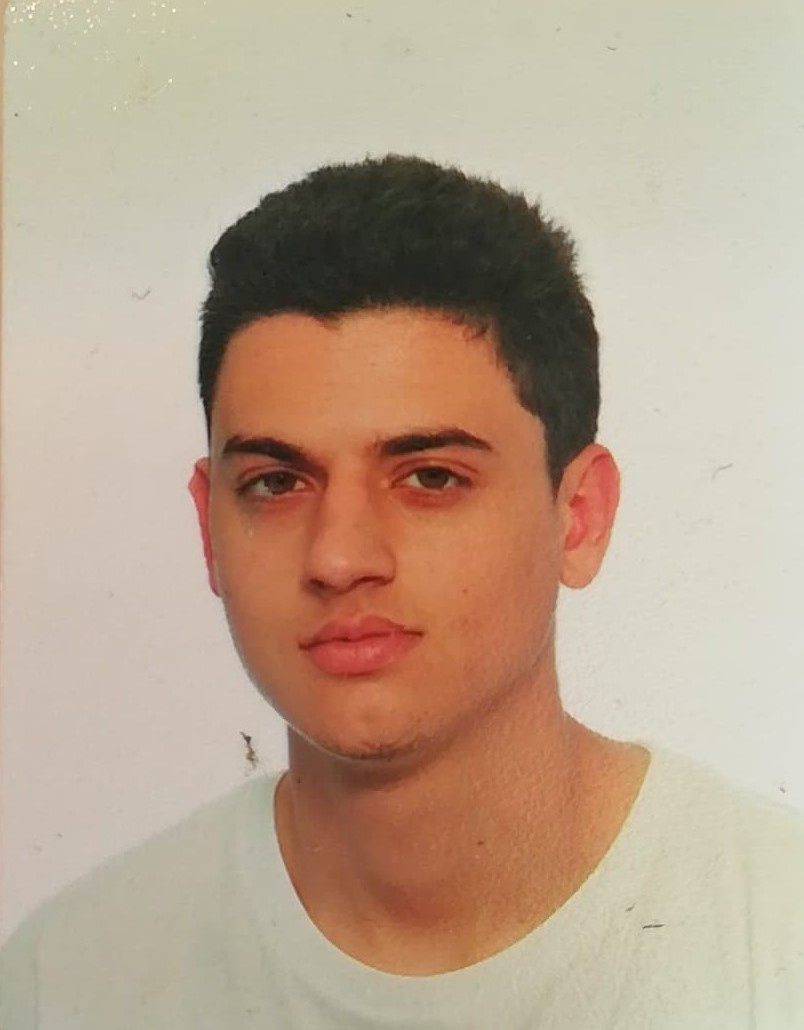
\includegraphics[width=0.25\textwidth]{PicProfil}
	\end{wrapfigure}
	Ο \textbf{Νικόλαος Γεωργόπουλος-Νίνος} είναι τριτοετής φοιτητής στο τμήμα Μηχανικών Ηλεκτρονικών Υπολογιστών και Πληροφορικής στο Πανεπιστήμιο Πατρών. Στη μέχρι τώρα πορεία του έχει αποκτήσει γνώσεις προγραμματισμού (\foreignlanguage{english}{Python, Java, C++, C}) και υπόβαθρο σε αλγοριθμικά και θεωρητικά θέματα των υπολογιστών. Παράλληλα στο πλαίσιο εκπόνησης εργασιών στα μαθήματα του προγράμματος σπουδών έχει αναπτύξει δεξιότητες συνεργασίας με άλλους μηχανικούς, κατανόησης σύνθετων προβλημάτων, σχεδιασμού λύσεων και υλοποίηση πρωτοτύπων. Επίσης, είναι ικανός να αναλαμβάνει εργασίες, τις οποίες ολοκληρώνει επιτυχώς, είτε αυτές είναι αυτούσιες ή μέρος μεγαλύτερων έργων. Τα ερευνητικά του ενδιαφέροντα περιλαμβάνουν τεχνολογίες ΙοΤ, δίκτυα \foreignlanguage{english}{5G} και κατανεμημένα συστήματα.
	
\end{document}
